% vim:set textwidth=100:
% vim:set fo+=t:

\documentclass[12pt]{article}

\usepackage{amsmath}
\usepackage[nofiglist,notablist]{endfloat}
\usepackage[usenames,dvipsnames]{color}
\usepackage{color}
\usepackage{authblk}
\usepackage{graphicx}
\usepackage{palatino}
\usepackage[activate={true,nocompatibility},final]{microtype}
\usepackage[super,sort&compress]{natbib}
\pagenumbering{arabic}
\parskip = 0.08in \parindent = 0.0in

% Custom macros for author comments
\newcommand{\Alberto}[1]{\color{ForestGreen}#1\normalcolor }
\newcommand{\Justin}[1]{\color{blue}#1\normalcolor}
\newcommand{\Arijit}[1]{\color{magenta}#1\normalcolor}
\newcommand{\Ken}[1]{\color{red}#1\normalcolor}

\author{Arijit~Roy}
\author{Alberto~Perez}
\author{Ken~A.~Dill}
\author{Justin~L.~MacCallum}
\affil{Laufer Center for Physical and Quantitative Biology\\
    and Departments of Physics and Chemistry\\
    Stony Brook University\\
    Stony Brook, NY 11794-5252.}

\title{Predicting the conformational preferences of proteins using a physics-based free energy
method}

\begin{document}

\maketitle


\section{Preparation of input model for chamelon sequences}

We prepared computer generated models in both $\alpha$ and $\beta$ conformation for all five chamelon sequences mentioned 
in the main text. Crystallographic structure of GA95 and GB95 sequence have $\alpha$ and $\beta$ fold respectively. When,
we attempt to prepare the $\alpha$ and $\beta$ fold with GA95 sequence we start with the crystallographic 
structure of GA95 and GB95 with GA95 sequence. However, we remove the sidechains at three mutated positions in both the fold 
and call the program SCWRL4 \cite{Krivov2009} to generate the sidechain conformation of the mutated residues and its neighbors. Followed by 
this step, we do long molecular dynamics
minimization to remove any possible bad contact. This procedure was followed to generate all $\alpha$ and 
$\beta$ conformations of five sequences that are used for free energy calculation.   


\begin{figure}
\includegraphics[width=5.6 in,height=5.3 in]{orban_perres_SI.pdf}
\label{fig:orban_full}
\caption{Per residue free energy calculation indicate significant differences of sidechain orientation of key amino acid residues. These amino acid
residues control the free energy equilibrium to either $\beta$ or
$\alpha$ conformation. All figures in the left are in $\beta$ conformation, whereas the right ones are in $\alpha$ conformation except in Figure (F).
Sidechains of hydrophobic residues Leu-7 in (A) and Ala-26 in (B) are oriented towards the protein interior in $\beta$ 
conformation. In such conformation they have hydrophobic interactions with other hydrophobic residues colored in white. In $\alpha$ conformation these residues are 
exposed to the protein surface. 
(C) Tyr-45 forms H-bond with Asp-47 with GB95 sequence and $\beta$ conformation. (D) Gln-11 and Glu-15 form a H-bond in $\beta$ conformation which is absent
in the $\alpha$ conformation. (E) Hydrophobic Ile-49 is exposed to the protein surface in $\beta$ conformation, whereas it is inside protein hydrophobic core in
$\alpha$ conformation. (F) Sidechain of Ile-30 is inside the protein hydrophobic core in as it has a smaller sidechain with GA95 sequence in $\alpha$ conformation. 
In contrast, Phe-30 with larger sidechain is exposed to the protein surface with GB95 sequence.}
\end{figure}

\begin{figure}
\begin{center}
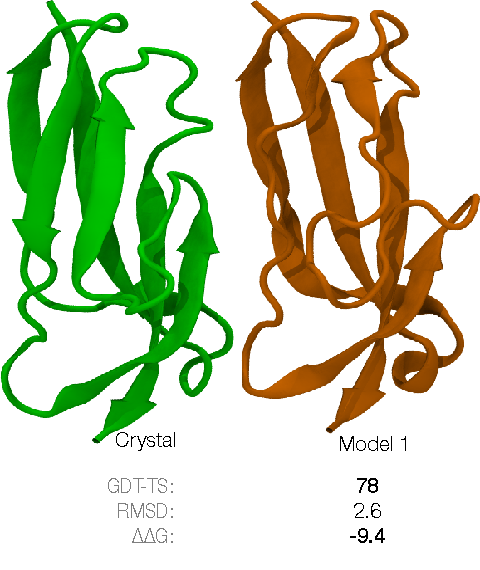
\includegraphics[width=3.6 in,height=3.4 in]{T0569.pdf}
\end{center}
\caption{Native and best model structure of a domain of adhesion exoprotein from Pediococcus pentosaceus (pdb id: 2KWY and CASP code: T0569).
The best model was from the group "Mufold".}
\label{fig:T0569}
\end{figure}


\begin{figure}
\begin{center}
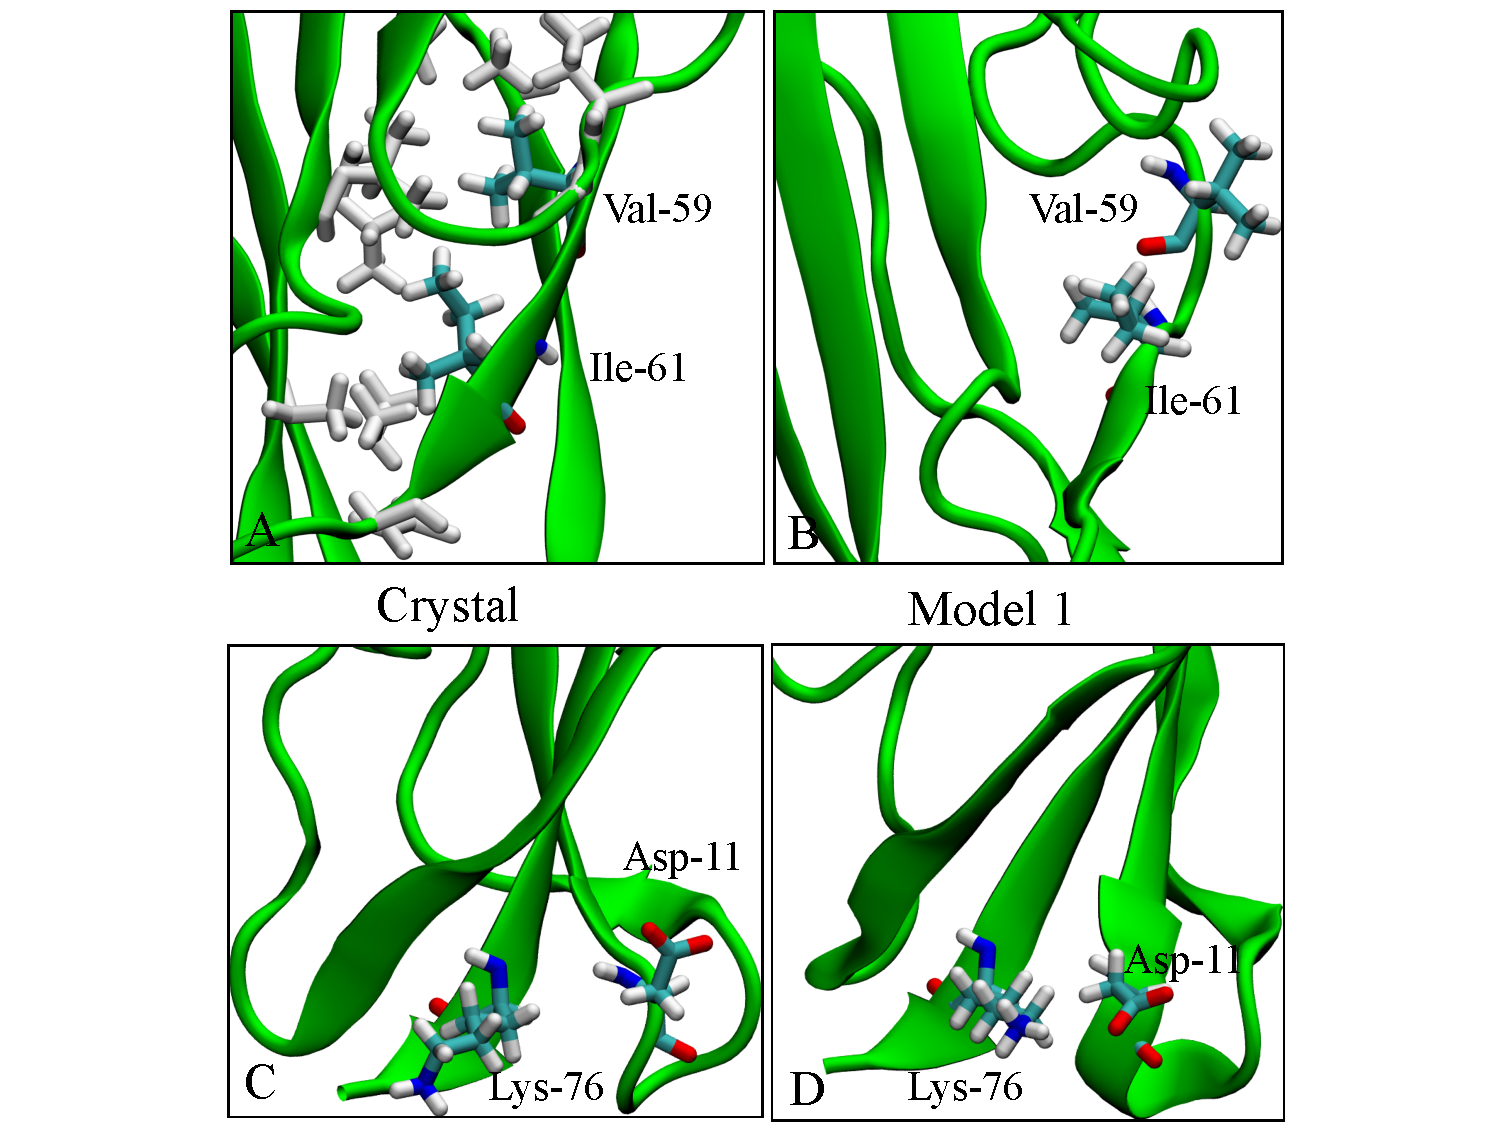
\includegraphics[width=5 in,height=4 in]{T0569_perres2.pdf}
\end{center}
\caption{Key differences between native crystal structure and the model as indicated by per residue free energy calculation.
The sidechain of hydrophobic residues, Val-59 and Ile-61 are oriented towards the protein hydrophobic core in (A) crystal 
structure, (B) exposed to the surfure in model. The beta sheet containing these residues is disordered in the generated model.
There is a H-bond between Lys-76 and Asp-11 in (D) model structure, which is absent in the (C) native structure.}
\label{fig:T0569_per_residue}
\end{figure}

\begin{figure}
\begin{center}
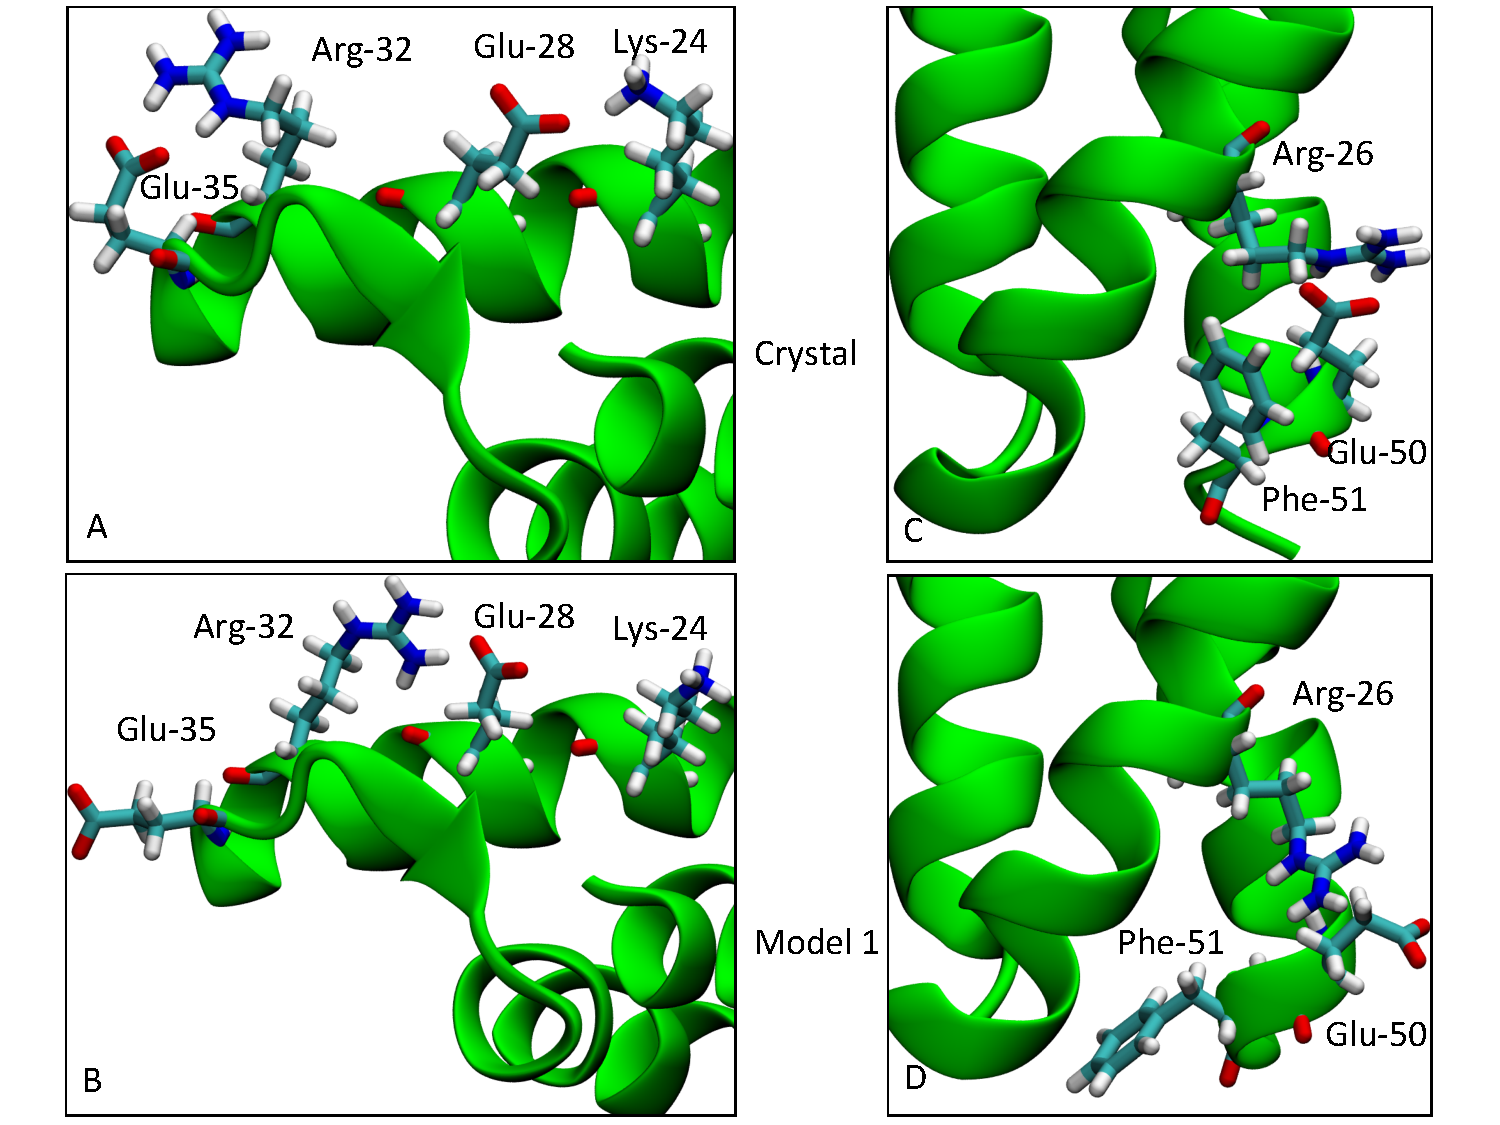
\includegraphics[width=4.9 in,height=4.0 in]{Target_538_compare.pdf}
\end{center}
\caption{Differences of the sidechain orientation in model 1 and crystallographic structure of CASP target T0538 as determined 
by per residue free energy calculation.  
(A) Two salt bridges between residues Glu-35-Arg-32 and Glu-28-Lys-24 exist in the native crystallographic structure. These are
absent in the model structure. Instead
(B) a new salt bridge is formed between residues Arg-32-Glu-28 in model. (C) Another salt bridge between
residues  Arg-26-Glu-50 in the native structure, (D) This salt bridge is absent in the model structure. In comparison to the crystallographic 
structure, orientation of Phe-51 differs in model1.}
\label{fig:T0538compare}
\end{figure}

\Ken{[This fig isn't very readable.  We need to focus into the sidechains, keeping only the nearby pieces of chain and leaving the rest out or making it fuzzy or something.  We need to see some point that you are making by looking at the figure.]}

\begin{thebibliography}{99}

\bibitem{Krivov2009}
Krivov, G.G.; Shapovalov, M.V.; Dunbrack, RL Jr. Improved prediction of protein side-chain conformations with SCWRL4.
Proteins. (2009) 77, 778-795.

\end{thebibliography}

%\end{suppinfo}
\end{document}
